\documentclass{beamer}
\usetheme{Berlin}
\usepackage{amsmath}
\usepackage{amsthm}
\usepackage{amssymb}
\usepackage{amsbsy}

\title{Inside-Out: Characterisation of Computed Tomography Noise in Projection and Image Space with Applications to 3D Printing}
\author{Sherman Ip}
\institute{University of Warwick}
\date{13th June 2016}

\AtBeginSection[]{
  \begin{frame}
      \tableofcontents[currentsection]
  \end{frame}
}

\DeclareMathOperator{\expfamily}{ExpFamily}
\DeclareMathOperator{\expectation}{\mathbb{E}}
\DeclareMathOperator{\variance}{\mathbb{V}ar}
\DeclareMathOperator{\cov}{\mathbb{C}ov}
\DeclareMathOperator{\corr}{\mathbb{C}orr}
\DeclareMathOperator{\bernoulli}{Bernoulli}
\DeclareMathOperator{\betaDist}{Beta}
\DeclareMathOperator{\dirichlet}{Dir}
\DeclareMathOperator{\bin}{Bin}
\DeclareMathOperator{\MN}{Multinomial}
\DeclareMathOperator{\prob}{\mathbb{P}}
\DeclareMathOperator{\trace}{Tr}
\DeclareMathOperator{\normal}{N}
\DeclareMathOperator{\gammaDist}{Gamma}
\DeclareMathOperator{\poisson}{Poisson}

\newcommand{\RSS}{\mathrm{RSS}}
\newcommand{\euler}{\mathrm{e}}
\newcommand{\diff}{\mathrm{d}}
\newcommand{\T}{^\textup{T}}
\newcommand{\dotdotdot}{_{\phantom{.}\cdots}}
\newcommand{\BIC}{\textup{BIC}}

\newcommand{\vect}[1]{\mathbf{#1}}
\newcommand{\vectGreek}[1]{\boldsymbol{#1}}
\newcommand{\matr}[1]{\mathsf{#1}}

\begin{document}

\frame{\titlepage}

\begin{frame}
\frametitle{Table of Contents}
\tableofcontents
\end{frame}

\section{Introduction}

\begin{frame}
\frametitle{3D Printing}
\begin{itemize}
	\item Quality control
	\item X-ray Computed Tomography
\end{itemize}
\begin{figure}
	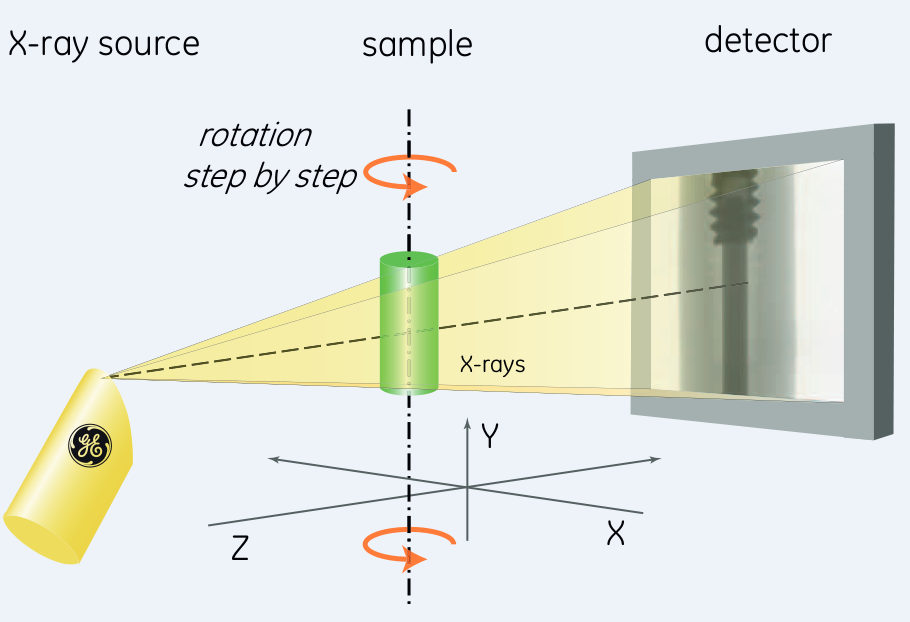
\includegraphics[width=0.5\textwidth]{figures/x_ray_ct.png}
	\caption{X-ray CT}
\end{figure}
\end{frame}

\begin{frame}
\frametitle{X-ray}
\begin{itemize}
	\item Bremsstrahlung radiation
	\item Characteristic radiation
\end{itemize}
\begin{figure}
	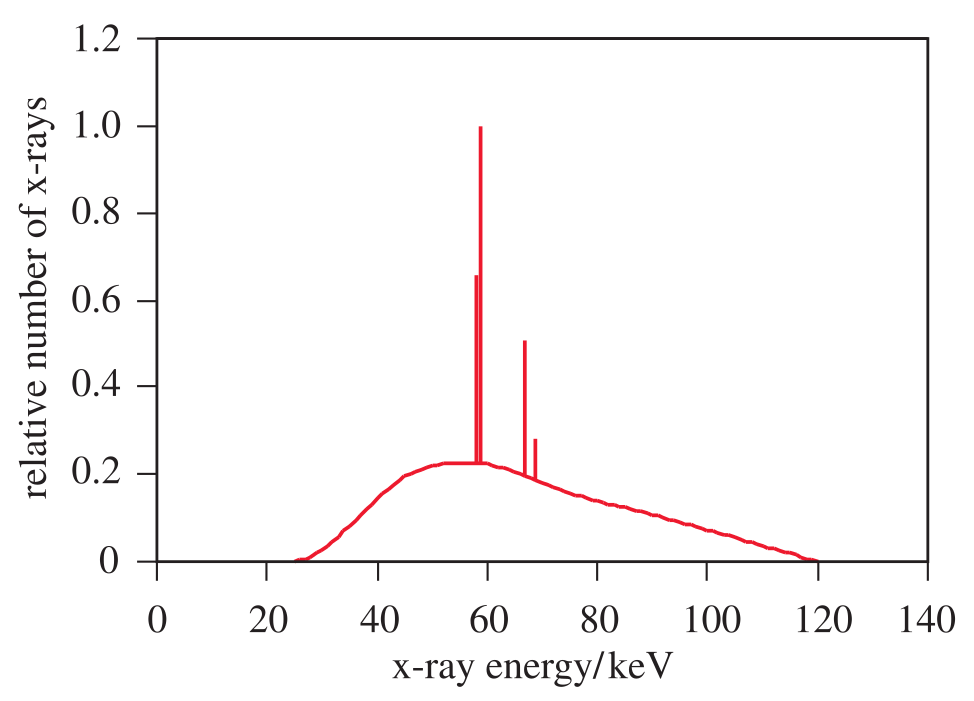
\includegraphics[width=0.5\textwidth]{figures/x_ray_spectrum.png}
	\caption{Energy spectrum}
\end{figure}
\end{frame}

\begin{frame}
\frametitle{Data}
\begin{itemize}
	\item 100 images
	\item 16-bit greyscale
	\item 1\,996 $\times$ 1\,996 pixels
	\item Stationary 3D printed cuboid
\end{itemize}
\end{frame}

\begin{frame}
\frametitle{Data}
\begin{figure}
	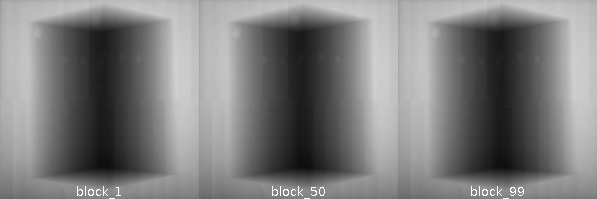
\includegraphics[width = \textwidth]{figures/block_montage.jpg}
	\caption{X-ray scans}
\end{figure}
\end{frame}

\begin{frame}
\frametitle{Data}
\begin{figure}
	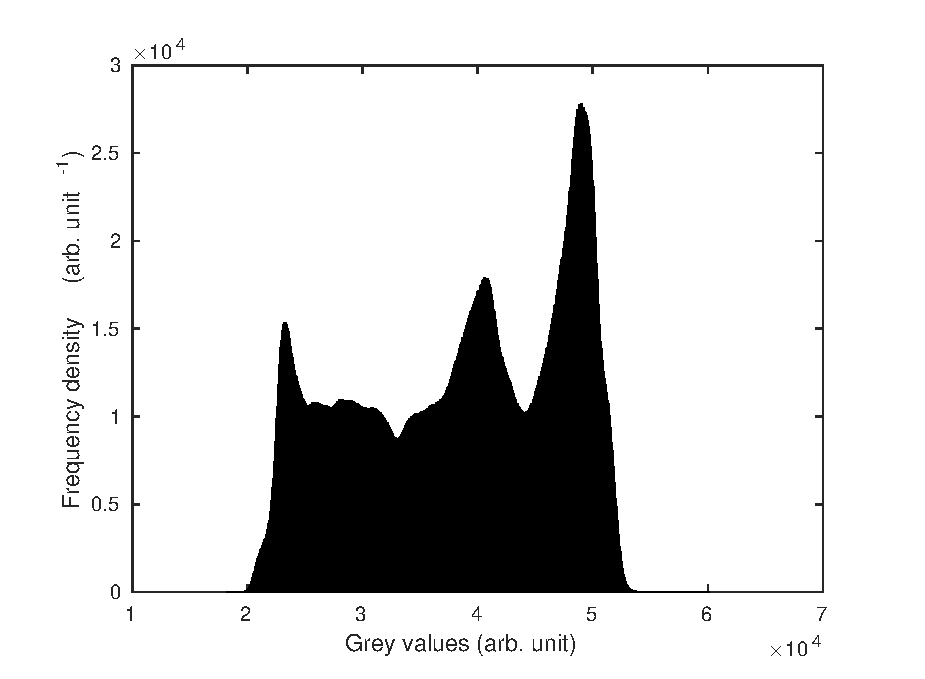
\includegraphics[width = 0.65\textwidth]{figures/block_histogram.eps}
	\caption{Histogram of grey values}
\end{figure}
\end{frame}

\begin{frame}
\frametitle{Aims}
\begin{itemize}
	\item Mean and Variance Relationship
		\begin{itemize}
			\item Supervised Learning
			\item Quantify uncertainty given a single CT scan
		\end{itemize}
	\item Latent Variable Models
		\begin{itemize}
			\item Unsupervised Learning
			\item Find sources of variance
		\end{itemize}
\end{itemize}
\end{frame}


\section{Mean and Variance Relationship}

\begin{frame}
\frametitle{Sample mean-variance}
\begin{figure}
	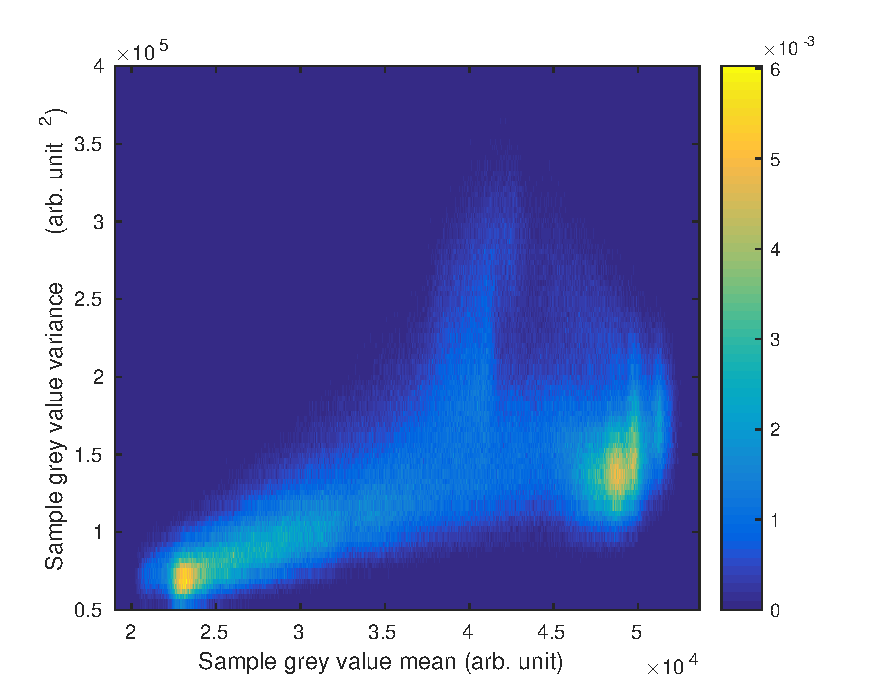
\includegraphics[width = 0.65\textwidth]{figures/meanVar/histogramHeatmap.eps}
	\caption{Frequency density plot}
\end{figure}
\end{frame}

\begin{frame}
\frametitle{Weighted Least Squares}
Deal with outliers
\begin{itemize}
	\item Weights proportional to the precision of the sample variance
\end{itemize}
\begin{equation}
w_i \propto \frac{1}{\left(S_i^2\right)^2}
\end{equation}
\end{frame}

\begin{frame}
\frametitle{Weighted Least Squares}
\begin{figure}
	\centering
		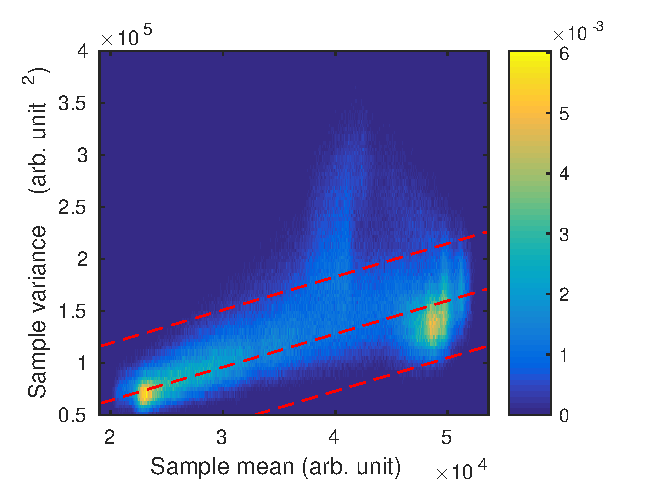
\includegraphics[width=0.3\textwidth]{figures/meanVar/order1.eps}
		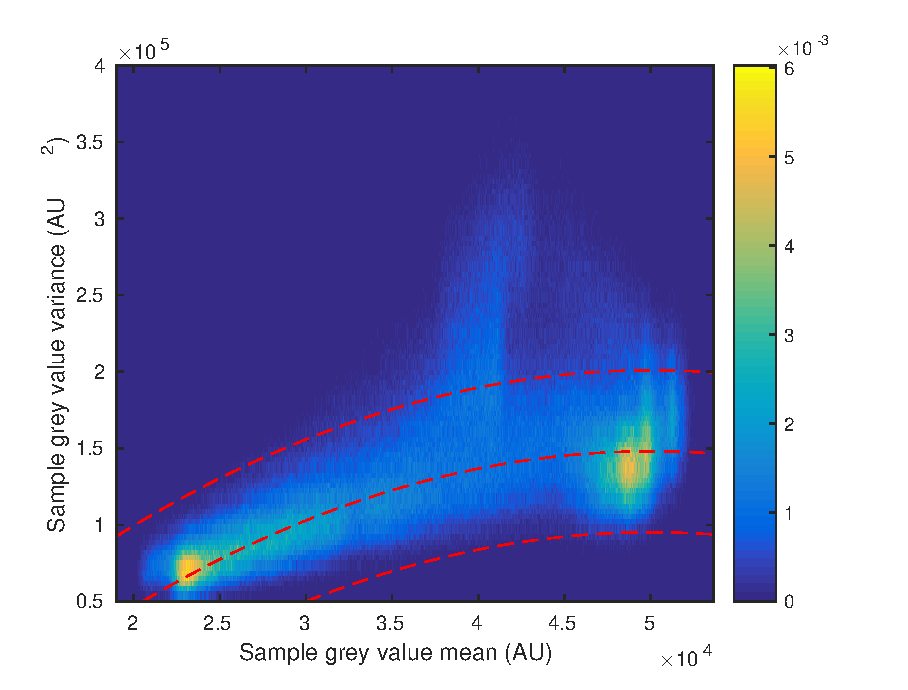
\includegraphics[width=0.3\textwidth]{figures/meanVar/order2.eps}
		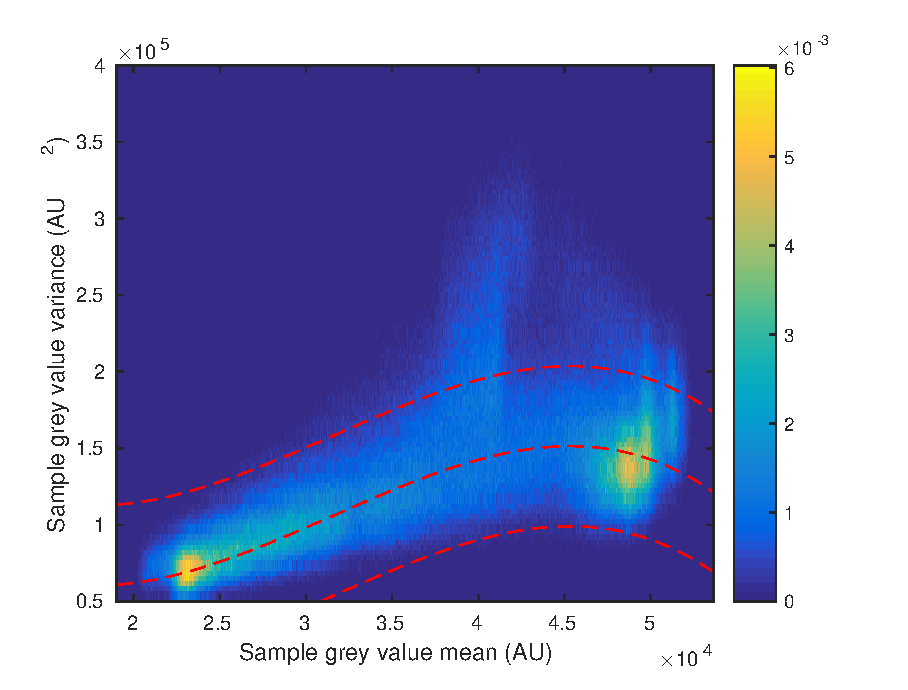
\includegraphics[width=0.3\textwidth]{figures/meanVar/order3.eps}
	\caption{Polynomial features}
\end{figure}
\end{frame}

\begin{frame}
\frametitle{Resampling}
\begin{figure}
	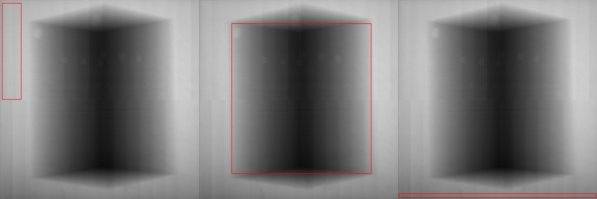
\includegraphics[width = \textwidth]{figures/meanVar/subsample_images.jpg}
	\caption{Resampling each material}
\end{figure}
\end{frame}

\begin{frame}
\frametitle{Resampling}
\begin{figure}
	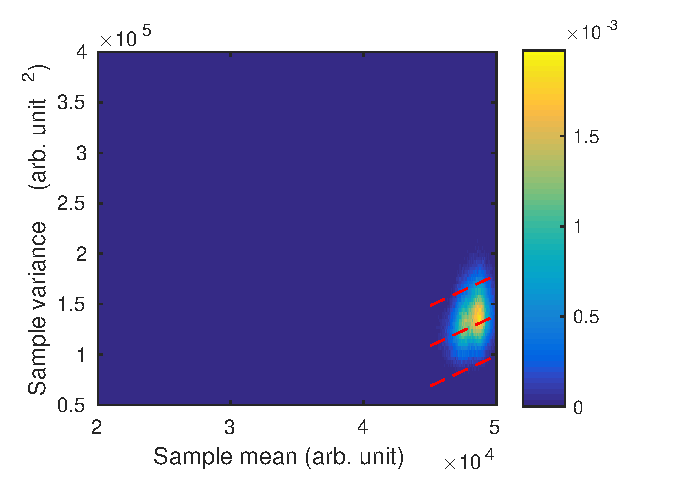
\includegraphics[width = 0.3\textwidth]{figures/meanVar/subsample_background1.eps}
	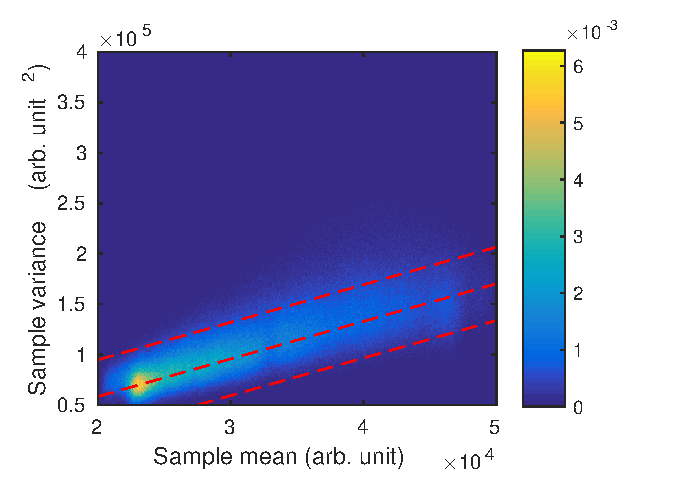
\includegraphics[width = 0.3\textwidth]{figures/meanVar/subsample_sample1.eps}
	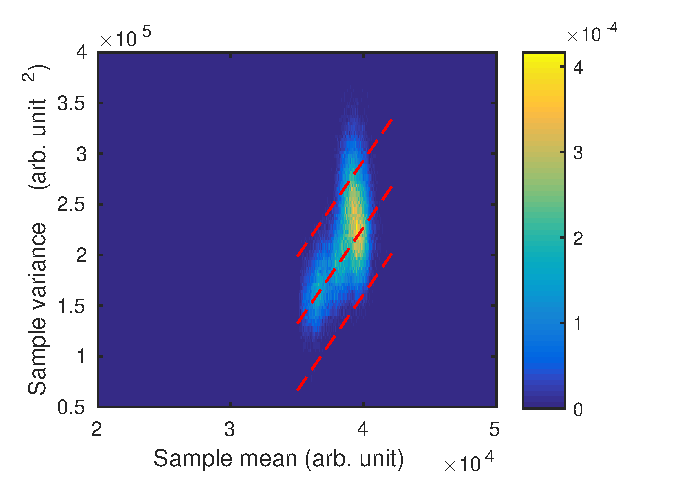
\includegraphics[width = 0.3\textwidth]{figures/meanVar/subsample_foam1.eps}
	\caption{Linear regression on each material}
\end{figure}
\end{frame}

\begin{frame}
\frametitle{Mixture of Linear Regression}
Attempt to capture 3 materials
\begin{equation}
Y_i\sim
\begin{cases}
\normal\left(\left(\vect{x}_i\right)\T\vectGreek{\beta}_1,\sigma_1^2\right) & \text{with probability }\pi_1\\ 
\normal\left(\left(\vect{x}_i\right)\T\vectGreek{\beta}_2,\sigma_2^2\right) & \text{with probability }\pi_2\\
\qquad\qquad\vdots\\
\normal\left(\left(\vect{x}_i\right)\T\vectGreek{\beta}_q,\sigma_q^2\right) & \text{with probability }\pi_q\\
\end{cases}
\end{equation}
Fit using EM algorithm.
\end{frame}

\begin{frame}
\frametitle{Mixture of Linear Regression}
\begin{figure}
	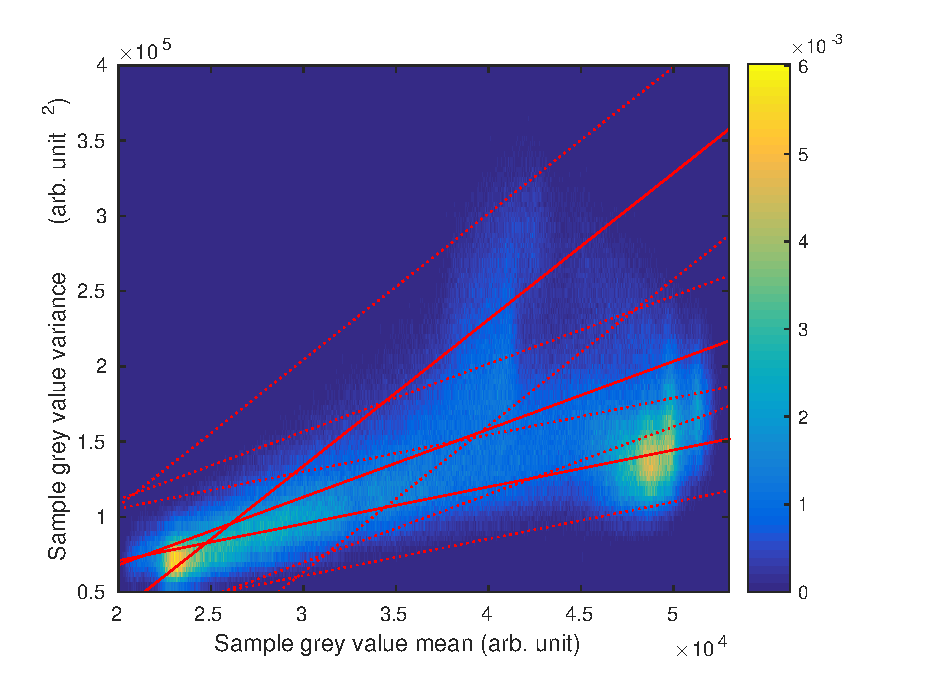
\includegraphics[width=0.65\textwidth]{figures/meanVar/mixture_histogram.eps}
	\caption{Mixture of Linear Regression}
\end{figure}
\end{frame}

\begin{frame}
\frametitle{Gaussain Weighted Least Squares}
Assign weights
\begin{equation}
w_i=\exp\left[-\frac{1}{2}\left(\frac{x_i-\mu_j}{\sigma}\right)^2\right]
\end{equation}
$\mu_j$ is some $k$ mean in the sample-mean space and $\sigma$ is some set constant.
\end{frame}

\begin{frame}
\frametitle{Gaussain Weighted Least Squares}
\begin{figure}
	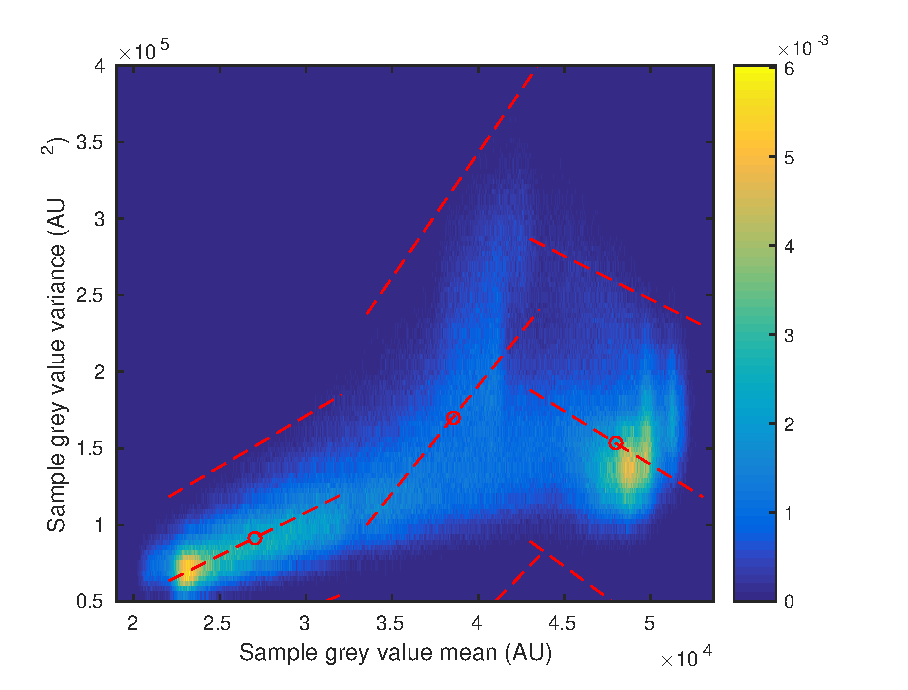
\includegraphics[width=0.3\textwidth]{figures/meanVar/gaussian_1.eps}
	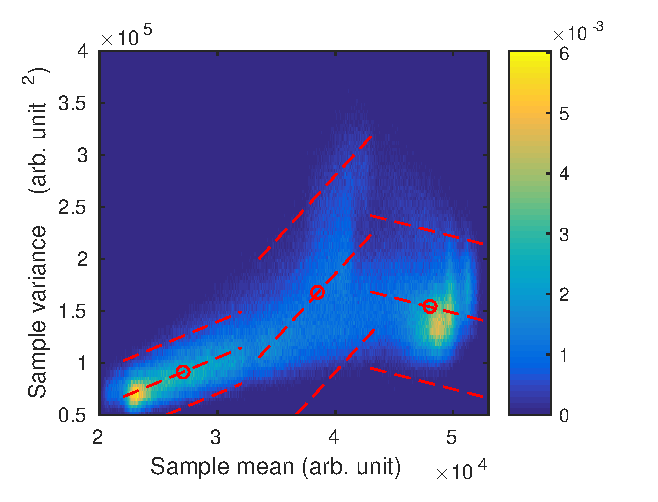
\includegraphics[width=0.3\textwidth]{figures/meanVar/gaussian_2.eps}
	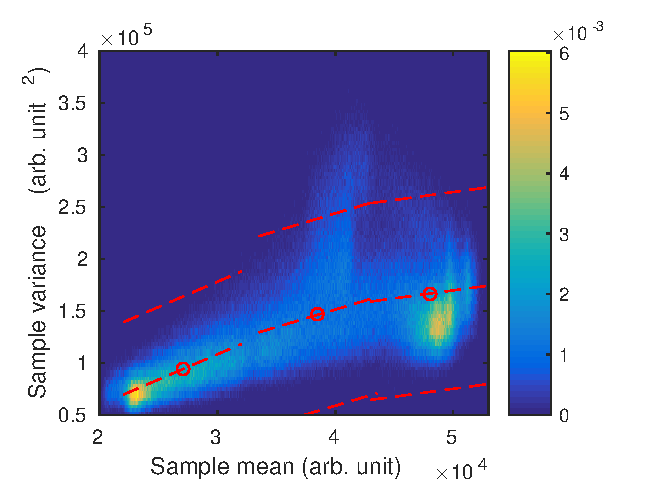
\includegraphics[width=0.3\textwidth]{figures/meanVar/gaussian_3.eps}
	\caption{Gaussian Weighted Least Squares $\sigma=\left\lbrace 10^2,10^3,10^4 \right\rbrace$}
\end{figure}
\end{frame}

\begin{frame}
\frametitle{Conclusion}
\begin{itemize}
	\item Material dependent
	\item Further work:
		\begin{itemize}
			\item Transformations
			\item Generalised Linear Models
		\end{itemize}
\end{itemize}
\end{frame}


\section{Latent Variable Models}

\begin{frame}
\frametitle{Principle Component Analysis}
Each pixel has random grey value. The eigendecomposition of the covariance matrix is
\begin{equation}
\matr{\Sigma} = \sum_{i=1}^{m} \lambda_i \vectGreek{\phi}_i \vectGreek{\phi}_i\T
\end{equation}
Shrink image to 100$\times$100.
\end{frame}

\begin{frame}
\frametitle{Principle Component Analysis}
\begin{figure}
	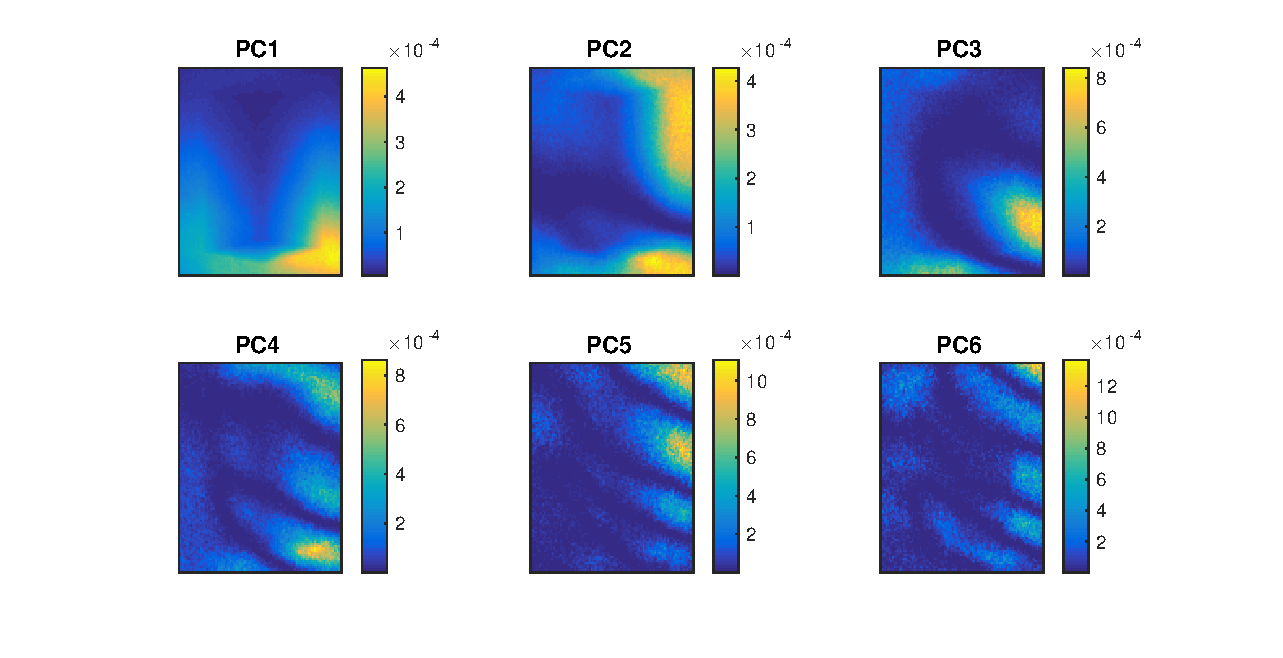
\includegraphics[width=\textwidth]{figures/initial_PCvariance.eps}
	\caption{Principle Components}
\end{figure}
\end{frame}

\begin{frame}
\frametitle{Factor Analysis}
$\vect{Y}$ is latent
\begin{equation}
\vect{Y}\sim\normal\left(\vect{0},\matr{1}\right)
\end{equation}
$\vect{e}$ is some uncorrelated random noise
\begin{equation}
\vect{e}\sim\normal\left(\vect{0},\matr{\Psi}\right)
\end{equation}
$\vect{X}$ is the observed grey values
\begin{equation}
\vect{X}=\matr{\Lambda}\vect{Y}+\vect{e}
\end{equation}
Fit using EM algorithm on shrunken 100$\times$100 images.
\end{frame}

\begin{frame}
\frametitle{Factor Analysis}
\begin{figure}
	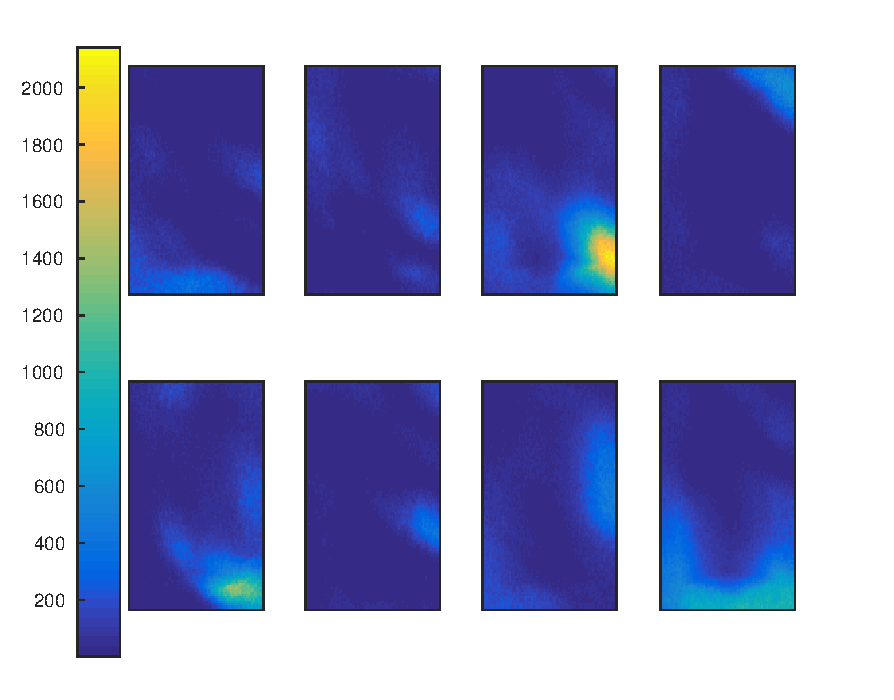
\includegraphics[width = 0.65\textwidth]{figures/initial_factor_factorNoise.eps}
	\caption{Factor Noise}
\end{figure}
\end{frame}

\begin{frame}
\frametitle{Factor Analysis}
\begin{figure}
	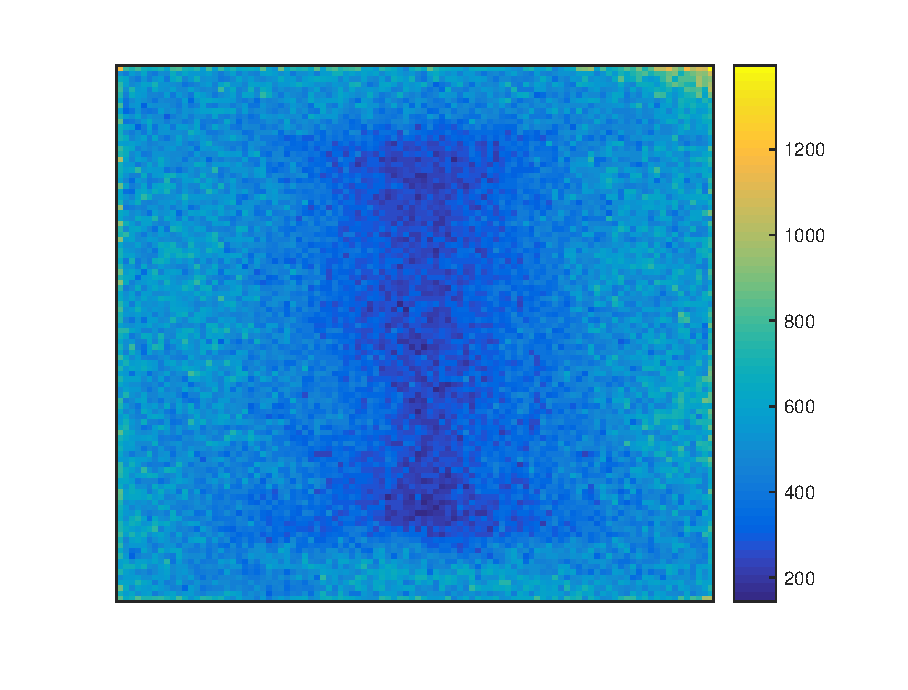
\includegraphics[width = 0.65\textwidth]{figures/initial_factor_instrinicNoise.eps}
	\caption{Instrinic Noise}
\end{figure}
\end{frame}

\begin{frame}
\frametitle{Compound Poisson}
$Y$ is the number of photons detected in a pixel
\begin{equation}
Y\sim\poisson(\nu \tau)
\end{equation}
$U$ is the total amount of energy recorded in a pixel
\begin{equation}
U|Y\sim\normal\left(
Y\mu,Y\sigma^2
\right)
\end{equation}
$X$ is the intensity recorded in a pixel
\begin{equation}
X|U\sim\normal\left(
\frac{\alpha}{\tau}U,\beta^2
\right)
\end{equation}
\end{frame}

\begin{frame}
\frametitle{Compound Poisson}
Marginalise over $U$ to get a one layer latent model
\begin{equation}
Y\sim\poisson(\nu\tau)
\end{equation}
\begin{equation}
X|Y\sim\normal\left(
\frac{\alpha\mu}{\tau}Y,\frac{\alpha^2\sigma^2}{\tau^2}Y+\beta^2
\right)
\end{equation}
\begin{block}{Remark}
There are 3 sources of variance
\begin{equation}
\variance[X] = \frac{\alpha^2\nu}{\tau}\left(\mu^2+\sigma^2\right)+\beta^2
\end{equation}
\end{block}
Fit using EM algorithm.
\end{frame}

\begin{frame}
\frametitle{Compound Poisson}
Easier for $\beta=0$. Problem: E step cannot be written down in closed form.
\begin{equation}
\expectation\left[Y|X=x\right]\propto
\sum_{y=1}^{\infty}\dfrac{\euler^{-\nu\tau}(\nu\tau)^{y}\tau}{y!\sqrt{2\pi}\alpha\sigma_i}y^{1/2}
\exp\left[-\dfrac{1}{2}\dfrac{\left(x-y\mu\alpha/\tau\right)^2}{\alpha^2y\sigma^2/\tau^2}\right]
\end{equation}
\end{frame}

\begin{frame}
\frametitle{Compound Poisson}
$\alpha=1,\tau=1,\nu=5,\mu=3,\sigma^2=0.1.$ Initialise using Poisson($\phi$).
\begin{figure}
	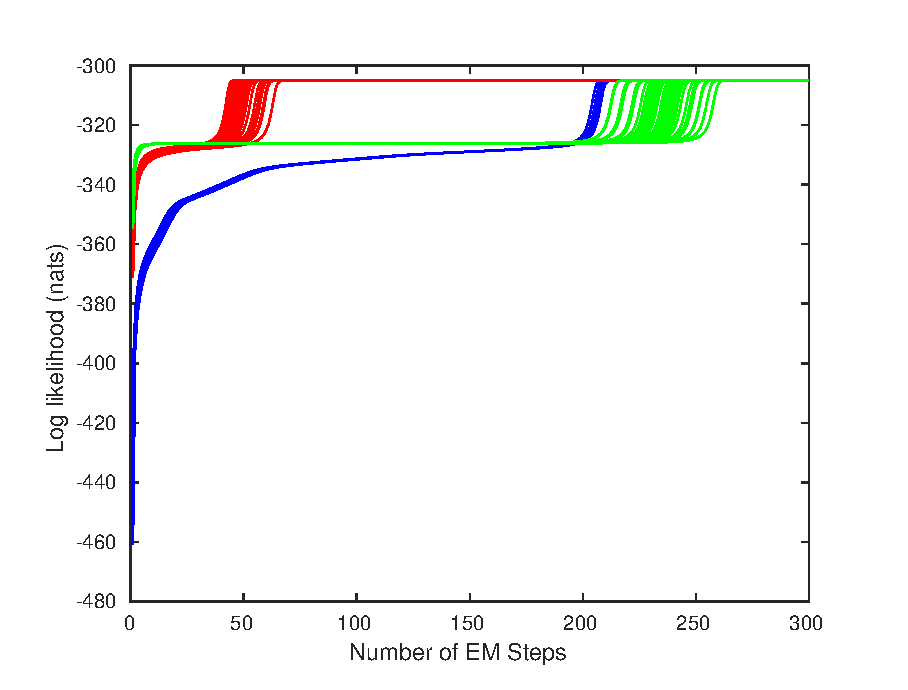
\includegraphics[width=0.5\textwidth]{figures/hierarchicalModel/EM_initial_lnL.eps}
	\caption{Blue: $\phi=1$, Red: $\phi=5$, Green: $\phi=9$}
\end{figure}
\end{frame}

\begin{frame}
\frametitle{Conclusion}
\begin{itemize}
	\item Variance dependent on each other.
	\item PCA and Factor Analysis needs to be scaled up.
	\item Fast approximations needed for Compound Poisson.
\end{itemize}
\end{frame}

\end{document}